\chapter{The thermal history of the universe}

\section{Introduction}
The goal of this chapter is that of going deeper in understanding something mentioned in the previous one: the thermal history of the Universe. In particular we want to understand how our universe tranformed from a hot, uniform soup of particles originated at the time of Big Bang, into the variety of atoms, molecules, planets, stars and galaxies that we see today. What we will cover in this section is the history of the universe up to when the first atoms, hydrogen, appeared; this epoch is really important in the study of cosmology because this is the time at which the Cosmic Microwave Background, which is one of the most solid observable evidences we have, originated. We shall see that the important epochs in the uiniverse history are characterized by the presence of different kind of particles and are characterized by different temperature scales $T$. In the first part of the lecture we will try to understand what is the meaning of these temperatures, i.e. how can we define the concept of temperature when 
we talk about the universe; in the following we will introduce some useful concepts to quantify the interactions between different kind of particles, and how these interactions depend strongly on the temperature scale. Finally, equipped with these tools, we will be able to study the most relevant steps in the history of the universe: the origin of nuclei, atoms and the cosmic microwave background. 

\section{The meaning of temperature}
You may recall that in some of the previous lectures we already encountered the concept of temperature, for example we saw several times that the measured temperature of the CMB (whatever this means) is $T=2.78$\,K: what is the precise meaning of that? We know that the CMB is made of photons, so what does it mean to associate a temperature to photons? We know from thermodynamics that, for a regular gas of particles (helium, hydrogen, air,...) the temperature is a measure of the average kinetic energy per particle $\langle U_{kin}\rangle$ according to the relation
\begin{equation}
\langle U_{kin}\rangle =\frac{3}{2}k_BT
\end{equation}
Where $k_B=1.38\cdot 10^{-23}$\,J/K is called Boltzmann constant; how can we extend this concept to photons? Photons are the particles which make up light and, for an e.m. (light) wave of frequency $\nu$, the photons which compose it carry a kinetic energy $U_{kin}=h\nu$ each ($h=6.63\cdot 10^{-34}$\,Js is called Planck constant). We are tempted to define temperature for photons in the same way as we did for the regular gas, and in some sense we can. We have to answer the question in an ensembleof photons (think about a oven for baking bread for example) at temperature $T$, what is their average kinetic energy? Statistical mechanics helps us in this one, stating that the probability of finding a particle with an energy $E$ in a system of temperature $T$ \textit{at thermal equilibrium} is proportional to $e^{-E/k_BT}$. This tells us that the prooability of finding $n$ photons of frequency $\nu$ in our oven is proportional to $e^{-nh\nu/k_BT}$. This allows us to compute the average number density and total 
energy density of all the photons of frequency $\nu$ as 
\begin{equation}
\langle n_\nu\rangle=\frac{1}{V}\frac{\sum_{n=0}^{\infty}ne^{-nh\nu/k_BT}}{\sum_{n=0}^{\infty}e^{-nh\nu/k_BT}}
\end{equation}
And the total energy density of these photons will be $u_\nu=h\nu \langle n_\nu\rangle$; performing the sum we get to an expression for the energy density $u_\nu$ of the photons of frequency $\nu$ in our oven as 
\begin{equation}
\label{planck}
u_\nu=\frac{8\pi h\nu^3}{c^3}\frac{1}{e^{h\nu/k_BT}-1}
\end{equation}
From this quantity we can derive the so called \textit{spectral radiance} $B_\nu(T)=\frac{c}{4\pi}u_\nu(T)$ which is the amount of energy of modes of frequency $\nu$, that crosses a unit area travelling in a certain direction, per unit time (it is measured in J s$^{-1}$ Area$^{-1}$ Hz$^{-1}$ steradian$^{-1}$); this is the quantity that is actually measured in experiments (like telesciopes, which measure the amount of energy received in a certain frequency band), when we look at our oven (or at the universe, which you may think of as a big, expanding oven) from inside. If we plot $B_\nu$ versus $\nu$ for different temperatures we obtain something like Figure \ref{blackbody1}.
\begin{figure}
\begin{center}
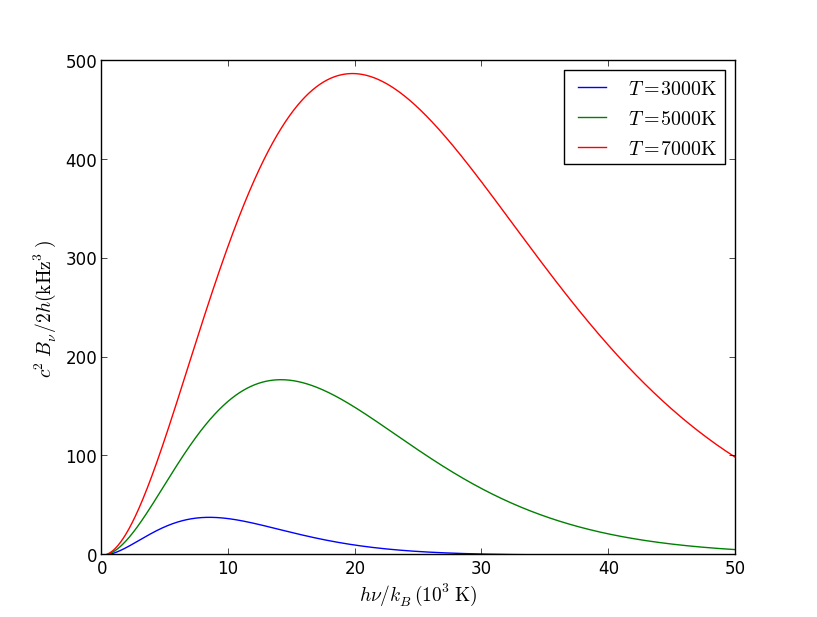
\includegraphics[scale=0.7]{Draw/blackbody.png}
\label{}
\end{center}
\caption{A plot of the spectral radiance $B_\nu$ versus $\nu$ for different temperatures $T$; you can notice that different curves peak at different frequencies. This fact is expressed by Wien's law that states $\frac{cT}{\nu_{peak}}=2.89\cdot10^{-3}\,$m$\cdot$K}
\label{blackbody1}
\end{figure}
You can see that, since observations today are able to probe a wide range of frequencies, looking at the shape of the curve and at the position of its peak, we are able to measure the temperature of our system (just choosing the best $T$ that fits our data); a system that has a spectral radiance which has a frequency distribution as in Figure \ref{blackbody1} is called a \textit{blackbody}. In nature there are a lot of systems that behave like blackbodies, in a very large range of temperatures, as outlined in Table \ref{blackbodies}
\begin{table}[htp]
\begin{center}
\begin{tabular}{|c|c|} \hline
\textbf{System} & \textbf{Blackbody temperatute} $T$ \\ \hline
The sun photosphere & 6000K \\ \hline
Your kitchen's oven & 450K \\ \hline
Earth's atmosphere & 300K \\ \hline
The Cosmic Microwave Background & 2.78K \\ \hline
Hawking radiation from black holes & Few fractions of K (too small to be detected) \\ \hline
\end{tabular}
\end{center}
\caption{Some physical systems that behave like blackbodies}
\label{blackbodies}
\end{table}
Now imagine that our universe (or big oven) expands: we already know that photons are redshifted, and this causes their energy to shift to low values. What effects does this have on the spectral radiance $B_\nu$? Clearly we have a redistribution of photon energies over all the spectral band, but remember that, when the universe's size grows by a factor $a$, \textit{all} the photons with frequency $\nu$ become photons with frequency $\nu'=\nu/a$. This means that, if we assume that no photons are created or destroyed
\begin{equation}
n_\nu d\nu=n_{\nu'}d\nu'a^3
\end{equation}
Now, remember from equation (\ref{planck}) that the photon number density is proportional to $n_\nu \propto \nu^2$ and that $\frac{d\nu}{d\nu'}=a$, and this means that $\frac{n_\nu}{\nu^2}=\frac{n_\nu'}{\nu'^2}$, which tells us that the spectral radiance of the expanding system \textit{has to maintain the shape of a blackbody} but in general with a new temperature $T'$ which can be derived observing that
\begin{equation}
\frac{1}{e^{h\nu/K_BT}-1}=\frac{1}{e^{h\nu'/k_B T'}}
\end{equation}
Which tells us immediately that $T'=T/a$; in this sense the universe \textit{cools down} as it expands; what does all this have to do with our study of cosmology? In 1990 the COBE satellite measured the spectral radiance of the Cosmic Microwave Backgronud, and their experimental data looked like Figure \ref{cmbspectral}
\begin{figure}
\begin{center}
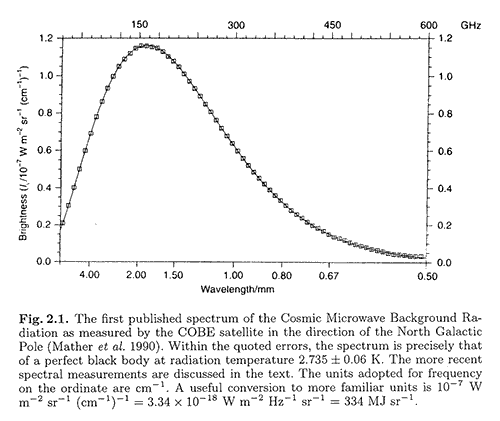
\includegraphics[scale=0.7]{Draw/cmbrad.png}
\label{}
\end{center}
\caption{Spectral radiance of the CMB as measured by the COBE satellite; the curve is consistent with a blackbody shape with a temperature of 2.78K. COBE experiment reference \url{http://lambda.gsfc.nasa.gov/product/cobe/c_images.cfm}}
\label{cmbspectral}
\end{figure}
This tells us two things: our universe today is \textit{very cold}, but when this CMB originated in the past, it could have been much hotter (we will see that it was at least 1000 times hotter. This radiation exibits a blackbody shape: it means that, when it originated in the past, the universe was in \textit{thermal equilibrium}; we will see that this is not true anymore today because the universe is almost neutral and hence ordinary matter has only very weak interactions with the photons. The picture in the subsequent paragraphs will be the following: the universe is composed by a lot of particles of different kind (photons, electrons, neutrinos, nuclei,...) that interact with each other with the three fundamental forces in the standard model (electromagnetic, strong force, weak force). Some of these interactions might be very efficient, some others less efficient, depending on the temperature of the system (we will outiline the important epochs in the \textit{thermal history of the universe} i.e. we will 
identify the temperatures at which each different interacton undergoes a drastic change in its efficiency). In principle each kind of particle can have its own temperature $T_i$, but all these temperatures are the same if all the species are in thermal equilibrium; for this reason, in the following we will refer to the \textit{temperature of the photons} as \textit{the temperature of the universe}, because photons are the particles which interact the most efficiently with matter, and are the last species to drop off thermal equilibrium. Before going into the actual thermal history of the universe, we need to understand better what does it mean that an interaction is \textit{efficient} or not; we will do this in the following paragraph. 

\section{When is an interaction considered efficient?}
\subsection{Particles number density}
\label{densities}
We have already seen in the previous lecture that the particles which compose the universe can be distinguished roughly in two big categories: hot particles that move close to the speed of light (photons and neutrinos) and cold particles which move at speeds much lower than $c$. The laws of thermodynamics tell us that these different kind of particles have very different number densities when they are in thermal equilibrium; in particular we have
\begin{itemize}
\item $n_{hot}(T)\propto T^3$ for hot particles; a particle species is considered hot, or relativistic, when its mass is very low compared to the typical energy scale, or $mc^2\ll k_BT$
\item $n_{cold}(T)\propto T^{3/2}e^{-mc^2/k_BT}$ for cold particles; a particle species is considered cold, or non relativistic when its mass is very big compared to the typical energy scale, or $mc^2\gg k_BT$. Note that for this main reason, and the exponential factor in $n_{cold}$ at equal temperature scales in general $n_{cold}\ll n_{hot}$
\end{itemize} 
\subsection{The strength of interactions}
We know that different kinds of particles can interact with each other according to the standard model, for example electrons interact with photons or neutrinos, protons interact with neutrons and they bind together to form nuclei, etc... How do we know how \textit{strong} each one of these interaction is? In particle physics the strength of an interaction process is quantified by a number, with measure units of an area, that is called \textit{cross section} and is usually denoted with the letter $\sigma$. To understand the precise meaning of this number, consider the following example in Figure \ref{crossec}
\begin{figure}
\begin{center}
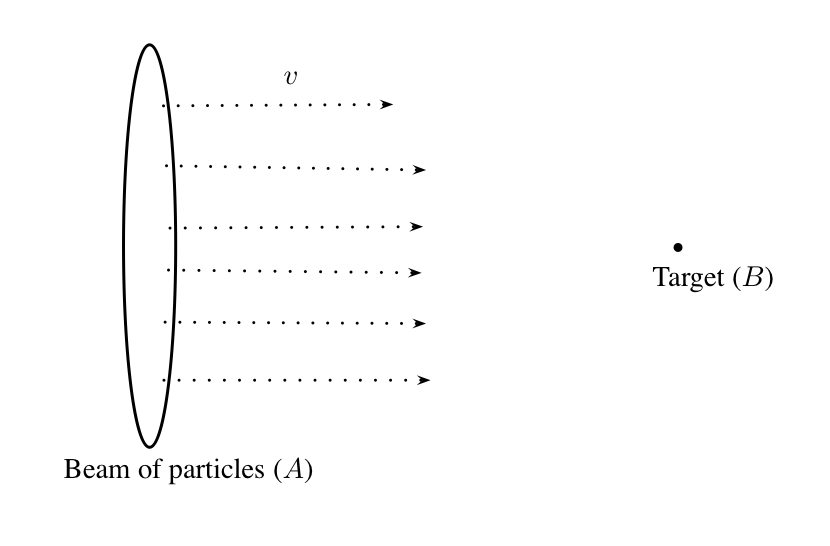
\includegraphics[scale=0.7]{Draw/cross_section.png}
\label{}
\end{center}
\caption{Illustrative example of an interaction of particles of species $A$ with particles of species $B$}
\label{crossec}
\end{figure}
Suppose we have a beam of particles of species $A$ that travel at velocity $v$ and are directed to a fixed target of particles of species $B$; a good way to characterize the strength of the interaction between $A$ and $B$ is to look at how many interactions will take place. If there are few the interaction is small, if there are many, the interaction is big; that's where the concept of cross section comes in hand. The cross section $\sigma_{AB}$ of an interaction process between $A$ and $B$ is defined as the \textit{effective area} that target $B$ offers to projectile $A$ for being hit. More quantitatively, if we call $\Sigma$ the numer of particles per unit area in the beam and $N_{int}$ the total number of interactions that take place, we should have
\begin{equation}
N_{int}=\Sigma \sigma_{AB}
\end{equation}
An important feature of this cross section is that it does not depend on the intensity of the beam or on the number of targets, but \textit{only} on the details of the interaction between $A$ and $B$ (it can depend on the energy scale of the collision though). To go onto more practical grounds, consider the following examples
\begin{itemize}
\item When we consider the collision of two solid balls of radius $R$ obviously the cross section associated with this process is $\sigma=\pi R^2$
\item Condider a photon ($\gamma$) - electron ($e^-$) at low energy (the so called \textit{Thomson scattering}): classical electrodynamics tells us that the cross section for this process is $\sigma_{th}=\frac{8\pi}{3}\left(\frac{e^2}{m_ec^2}\right)^2\approx0.66\cdot 10^{-28}\mathrm{m}^2$. The quantity $r_e=\frac{e^2}{m_ec^2}\sim 10^{-14}$m has dimensions of length and can be interpreted as the effective size of an electron. Note that this effective size does not have an absolute meaning (you won't be able to measure it with a ruler), but has only meaning in quantifying the interaction between electrons and photons
\item A photon - electron interaction at high energy (\textit{Compton scattering}) $\epsilon \gg m_ec^2$; the cross section for this process computed in full quantum electrodynamics is 
\begin{equation}
\sigma_{comp}\approx \pi r_e^2\left(\frac{\ln{\frac{2\epsilon}{m_ec^2}}}{\frac{\epsilon}{m_ec^2}}\right)
\end{equation} 
\item A neutrino ($\nu$) - electron interaction in neutrino energy range $E_\nu\approx 1$MeV has a cross section 
\begin{equation}
\label{neutel}
\sigma_{e\nu}\approx 10^{-48}\mathrm{m}^2\left(\frac{E_\nu}{1\mathrm{MeV}}\right)
\end{equation}
Note that, since this is a weak nuclear interaction process, its cross section is much smaller than a typical electromagnetic cross section $\sigma_{th}$
\item A typical neutron ($n$) - proton ($p$) nuclear collision has a cross section of $\sigma_{np}\approx 10^{-28}$m$^2$ 
\end{itemize} 
\subsection{Efficiency of reactions}
Now that we know how to quantify the \textit{strength} of particle interactions, we have to understand when a particular reaction is considered efficient in cosmological contexts: the fact that an interaction is strong (big $\sigma$), it doesn't mean that the same interaction is efficient. For example if the particles' densities are low, despite of the big cross section, there will be very few interaction events. How do we combine the density and cross section informations to get a good distinguishing criterion? Consider again Figure \ref{crossec}: suppose the impacting beam is composed by particles that travel at velocity $v$ and have a number density $n$; let be $\sigma$ the cross section of this particular interaction. You can convince yourselves that the quantity
\begin{equation}
\tau_{int}=\frac{1}{n\sigma v}
\end{equation} 
has the dimensions of time and represent the average time that elapses by two distinct interaction events; this average time depends jointly on the strength of the interaction and the reactants abundances. Now, remember that both $n,\sigma$ and $v$ depend on the temperature of the system (the equilibrium number densities and average velocities depend on $T$, but the temperature sets also a typical energy scale $E\sim k_BT$, on which the cross section in general depends), so in the end $\tau_{int}$ is a function of $T$. If this timescale is too big and the universe expands too fast bringing all the particles far from each other, clearly the reaction becomes inefficient. The timescale for the universe's expansion is set by the Hubble time, the inverse of the Hubble parameter $t_H=H^{-1}$; since $H$ depends on redshift, and hence on the temperature of the universe (through $T(z)=T_{CMB}/1+z$), we can say that $t_H$ depends on temperature too. We will say then that a reaction is \textit{efficient} if its 
timescale $\tau_{int}$ is much lower than the expansion timescale ($\tau_{int}\ll t_H$). Clearly at the big bang the universe is infinitely hot so all reactions will be efficient and all species will be at thermal equilibrium; for each reaction though, there will be a critical temperature $T_c$ at which $\tau_{int}(T_c)=t_H(T_c)$; below this temperature the reaction will become inefficient. If a particle species has no efficient interactions with the all the other species, it will drop out of thermal equilibrium. Photons are the last one dropping out of equilibrium, and when this happens the CMB is originated: the final goal of this chapter will be understanding when precisely does this happen. 

\section{The important epochs in the universe's life}
In the previous section we saw that a particular interaction process with energy dependent cross section $\sigma(E)$ becomes inefficient when the interaction timescale
\begin{equation}
\tau_{int}(T)=\frac{1}{n(T)\langle\sigma v\rangle_T}
\end{equation}
Becomes bigger than the expansion timescale $t_H=H^{-1}$; roughly speaking, $\tau_{int}$ becomes big when the cross section, the typical velocity, or the number density become small; if a particle species has no effective interaction with the other species, it drops out of thermal equilibrium, or it \textit{decouples}. Based on these considerations we are able to make two important observations:
\begin{itemize}
\item Neutrinos are capable to interact via the weak nuclear force only, their typical interaction cross section is really small, so it is likely that they are the first particle species to drop out of thermal equilibrium; this is precisely what happens
\item Photons have large cross sections (because they interact electromagnetically), the highest speed of all (they travel at the speed of light) and the highest number density (which scales as $T^3$, contrary to other non relativistic species, for which it is depressed by $e^{-mc^2/k_BT}$). For these reasons, it is likely that they are the last species to decouple; when this happens, the CMB is originated. 
\end{itemize}
\subsection{An unknown era}
The universe after the big bang started out really hot, all interaction processes were really efficient and all particles were in thermal equilibrium and could be described in terms of an unique temperature $T$; we don't know more about this period of time, when say $k_BT\gtrsim 1$GeV, because the theoretical tools to understand physics at such high energy scales (namely electroweak theory and quantum chromodynamics) are still under developement. We believe anyway that at a certain point the universe did undergo some kind of phase transition from being a hot soup of quark and gluons (a kind of quark/gluon plasma) to a stage where quarks became confined to form protons and neutrons. This quark/gluon plasma stage constitutes a very active branch of nuclear physics research today. 
\subsection{Neutrinos leave the party}
As said before, neutrinos are the first species to leave thermal equilibrium, because they interact so weakly with the rest of matter; the main process which keeps them coupled is scattering with electrons
\begin{equation}
\nu + e^- \rightarrow \nu + e^-
\end{equation}
With a cross section that scales roughly as (\ref{neutel}); we will be very qualitative in the following, because the computations needed to show the results presented are often lengthy and most of the time require computer algorithms to solve equations numerically. The results of these calculations is that, for this particular process $\tau_{int}\sim t_H$ when $k_BT\sim 1$MeV. At this point neutrinos decouple from the rest of species, and their temperature evolves independently without caring to what happens to the other species, as
\begin{equation}
k_BT_\nu(a)=1\mathrm{MeV}\frac{a(1\mathrm{MeV})}{a}
\end{equation}
The fact that neutrinos decouple means that they originate a sort of background radiation, called \textit{cosmic neutrino background} (or CNB) that free streams towards us; we can estimate the temperature of this radiation knowing the temperature of the CMB. Shortly after  neutrino decoupling, the electron positron annihilation process
\begin{equation}
e^+ + e^- \leftrightarrow \gamma+ \gamma
\end{equation}
becomes really efficient and gets heavily shifted to the right, adding extra photons to the budget; this means that the photon temperature grows (along with the temperature of all the species coupled to them; the neutrino temperature however does not grow, because they are alread decoupled); this heats up the photons by roughly a factor $\sqrt[3]{\frac{11}{4}}$ with respect to neutrinos. We can then estimate that today we expect a temperature
\begin{equation}
T_{CNB}=\sqrt[3]{\frac{4}{11}}T_{CMB}\approx 1.98\,\mathrm{K}
\end{equation}
This corresponds to an energy scale $k_BT_{CNB}\sim 10^{-4}$eV for the neutrinos, which is below any realistic detection threshold for state of art neutrino experiments (which are able to detect neutrinos with energies $\gtrsim 1$keV); unfortunately then there is no realistic hope to detect this cosmic neutrino background in the near future. 
\subsection{The first three minutes: primordial nucleosynthesis}
After the electron neutrino scattering becomes inefficient, neutrinos are still weakly coupled to neutrons and protons via the reactions 
\begin{equation}
\label{proton1}
n+e^+\leftrightarrow p+\bar{\nu}_e
\end{equation}
\begin{equation}
\label{proton2}
n+\nu_e\leftrightarrow p+e^-
\end{equation}
\begin{equation}
n\leftrightarrow p+e^-+\bar{\nu}_e
\end{equation}
The first two reactions become inefficient soon after the neutrino decoupling, precisely after $k_BT\lesssim 0.5$MeV (which corresponds roughly to 1\, second after the Big Bang); the last reaction however may potentially cause a problem. This is not a collision reaction, but rather a decay reaction in which, due to the fact that the neutron is slightly heavier than the proton ($m_n\sim m_p\sim 1$GeV but $m_n-m_p\approx$1.29\,MeV), a neutron can decay and produce lighter particles. The mean lifetime for this decay process is $\tau_n=$15\,minutes. This tells us that, if there is any hope at all to form heavier nuclei (such as deuterium and helium) via strong nuclear interactions, they better form before 15 minutes from the Big Bang, otherwise there may be no neutrons left to bind! Let's see if this is the case. Consider a generic reaction 
\begin{equation}
1+2\leftrightarrow 3+4
\end{equation}
which has associated a cross section $\sigma_{12}$; let's focus on species 1. We want to write down a differential equation for the evolution of its number abundance $n_1$; if there were no interactions, its number density would just decrease due to the fact that the universe is expanding and hence some dilution occurs according to the relation 
\begin{equation}
\label{ateq}
\frac{dn_1}{dt}=-3\frac{\dot{a}}{a}n_1=-3Hn_1
\end{equation}
Due to the interaction with species 2 though,m there might be some injections/subtractions of particles of type 1 in the reaction, quantified by the cross section $\sigma_{12}$ according to 
\begin{equation}
\label{balancenoneq}
\frac{dn_1}{dt}+3Hn_1=n_1^0n_2^0\langle \sigma_{12}v\rangle\left[\frac{n_3n_4}{n_3^0n_4^0}-\frac{n_1n_2}{n_1^0n_2^0}\right]
\end{equation} 
Where $n_i^0$ are the equilibrium number densities as seen in section \ref{densities}; note that the right hand size is close to zero when the reaction is inefficient ($H\gg n\sigma v$) or when the system is at equilibrium $n_i=n_i^0$. In both these cases the system is simple to solve because (\ref{ateq}) has a solution $n_1\propto a^{-3}$; the complicated stage is solving (\ref{balancenoneq}) when the right hand side is non negligible. Usually this can be done only numerically with a computer algorithm, writing down an equation similar to (\ref{balancenoneq}) for each species, when all the cross sections are known. If we apply this method to one of the weak neutron proton reactions (\ref{proton1}) or (\ref{proton2}),along with the information we know about the neutron lifetime, and use a computer to solve for the neutron abundance $X_n\equiv \frac{n_n}{n_n+n_p}$, we obtain a behavior similar to the one outlined in Figure \ref{abun}
\begin{figure}
\begin{center}
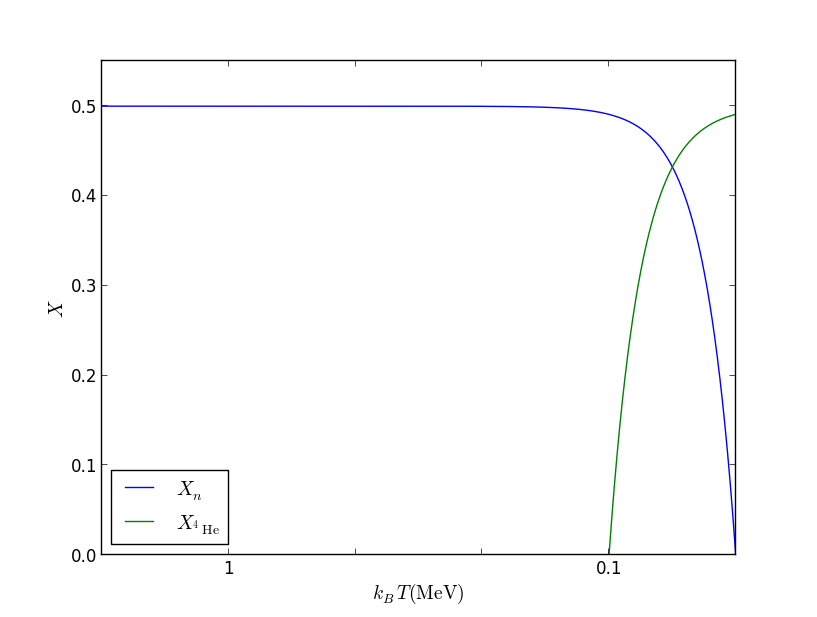
\includegraphics[scale=0.7]{Draw/abundances.png}
\label{}
\end{center}
\caption{Fractional abundances $X_i=n_i/(n_i+n_p)$ of neutrons and $^4$He nuclei as a function of the photon temperature $T$, as results from the numerical solution of the abundance equations (\ref{balancenoneq})}
\label{abun}
\end{figure}
This tells us that the neutron abundance starts to drop dramatically after $k_BT\lesssim 0.1$MeV, due to the weak interactions becoming inefficient in producing new neutrons to replace the ones that decay. Our only hope for forming heavier nuclei, then, is that by this time strong nuclear processes are efficient enough to bind the protons with the neutrons that are left. This is done mainly via the strong process
\begin{equation}
p+n\leftrightarrow D + \gamma
\end{equation}
Where $D$ indicates deuterium, a nuclear bound state between a neutron and a proton. When this reaction is at equilibrium, the deuterium abundance has to obey the thermodynamic equation
\begin{equation}
\label{deuterium}
\frac{n_D}{n_nn_p}=\frac{3}{4}\left(\frac{m_Dh^2}{2\pi k_Bm_nm_p T}\right)^{3/2}e^{(m_n+m_p-m_D)c^2/k_BT}
\end{equation}
Where $B_D=m_n+m_p-m_D=2$MeV is the binding energy of deuterium; for the purpose of this section we will make the crude estimate (for $k_BT\lesssim 0.1$MeV) $n_n\sim n_p \sim\eta_b n_\gamma$. With $n_\gamma \propto T^3$ and $\eta_b\approx 10^{-9}$ is measured from CMB experiments which tell us that there are roughly one billion photons for every baryon in the universe. This allows us to write the approximate equation, starting from (\ref{deuterium})
\begin{equation}
\frac{n_D}{n_p}\sim \eta_b\left(\frac{k_B T}{m_p c^2}\right)^{3/2}e^{B_D/T}
\end{equation}
If we try to see when a substantial amount of deuterium is produced we try to solve this equation for $T$ setting $n_D/n_p=1$ and, again using numerical methods, we get that this happens when $k_B T\approx k_B T_{nucl}=0.07$\,MeV. This corresponds to a redshift $1+z_{nucl}=\frac{T_{nucl}}{T_{CMB}}\approx 2\cdot 10^8$ which translated in time in the $\Lambda$CDM model corresponds to 3 minutes after the Big Bang. We can consider ourselves very lucky then: our universe is made in such a way that the strong nuclear interaction is efficient enough to store most of the neutrons into deuterium in just three minutes, just about in time before all the neutrons decay (which occurs after 15 minutes). If we look again at Figure \ref{abun} we see that that at this time the neutron proton fraction has dropped roughly to $n_n/n_p=1/7$. Now that the neutrons are safely stored into deuterium, the following reactions can occur to produce a heavier nucleus, helium 4, which is formed via
\begin{equation}
D+D \rightarrow n + ^3\mathrm{He}
\end{equation}
\begin{equation}
^3\mathrm{He}+D \rightarrow p + ^4\mathrm{He}
\end{equation}
Helium for is a very stable nucleus, with a binding energy of $B_{^4\mathrm{He}}=28$MeV and it takes about 20 minutes to accumulate in a substantial fraction; once the helium production is over, our current estimates state that helium can account for the 25\% of the mass of baryonic (non dark) matter. These processes of primordial nucleosynthesis cannot form nuclei which are heavier than helium because formation processes like 
\begin{equation}
^4\mathrm{He} + ^4\mathrm{He} +^4\mathrm{He} \rightarrow ^{12}\mathrm{C}
\end{equation}
which can form carbon (the next stable nucleus), require a much bigger helium abundance than 25\% in order to be efficient. For these heavier elements to be formed we have actually to wait for the first collapsed structures to form; when the first stars are formed, carbon can be produced via thermonuclear fusion processes which occur in the core of stars. 
\subsection{The origin of the CMB}
In the previous paragraph we saw that the first light nuclei (which consist in deuterium and helium 4) form respectively after 3 and 20 minutes via strong interactions, solving the problem weak interactions may cause when making the neutron decay with a lifetime of 15 minutes. What is the next step? At this stage in the life of the universe, photons are still tigthly coupled to charged matter, which includes electrons and charged nuclei. After nucleosynthesis, nothing really interesting really happens to this ensemble of particles,which consists in a hot plasma of nuclei and electrons not bound together, immersed in this sea of photons, cooling down as the universe expands. To wait for something actually interesting to happen actually we have to wait other 300,000 years, after which the universe has cooled a sufficient amount to allow electrons bind with protons and charged nuclei to form neutral atoms; this epoch is called \textit{recombination}. In a very similar way as neutrons and protons combine via 
strong nuclear interactions to form deuterium nuclei, protons and electrons can combine to form neutral hydrogen atoms via the electromagnetic reaction
\begin{equation}
p+e^-\leftrightarrow H + \gamma
\end{equation}
An important difference with the previous process is that the binding energy of the hydrogen atom $B_H=m_e+m_p-m_H=13.6$eV is much lower than the binding energy of deuterium nuclei; this is why it's much easier to break an electromagnetic electron proton bond, and a much lower temperature is required for this bond to resist and hold atoms together. Following the guideline of equation (\ref{deuterium}), when the reaction is at equilibrium, we can write a similar relation for electron and hydrogen abundances
\begin{equation}
\frac{n_H}{n_en_p}=\left(\frac{m_Hh^2}{2\pi k_Bm_em_p T}\right)^{3/2}e^{T^*/T}
\end{equation}
With $T^*=B_H/k_B=1.6\cdot 10^5$\,K; now, if we define the ionized fraction of hydrogen $x$ as $n_p=x(n_H+n_p)$ and if we make the simplification $n_e\sim n_p\sim \eta_b n_\gamma$, we can derive a simplified equation for $x$ as a function of temperature, in an analogous way as we did before we did before
\begin{equation}
\frac{1-x}{x^2}\approx 10^{-8}\left(\frac{k_BT}{m_ec^2}\right)^{3/2}e^{T^*/T}
\end{equation}
To get an idea on when recombination occurs, we want to see at which temperature the ionized fraction drops very low, and the hydrogen atoms are dominating in number over the unbound protons; if we set a reference as $x+10^{-3}$, we have to solve for $T$ the equation
\begin{equation}
\left(\frac{k_BT}{m_ec^2}\right)^{3/2}e^{T^*/T}=10^{14}
\end{equation}
Again we can use a computer to do this, but a good approximation, just to set the order of magnitudes is the following
\begin{equation}
T(x=10^{-3})\equiv T_{rec}\approx \frac{T^*}{14\ln{10}+\frac{3}{2}\ln{\left(\frac{m_ec^2}{k_BT^*}\right)}}\approx 3000\, \mathrm{K}
\end{equation}
When the temperature drops below this value, the reactions that keep the photons coupled to charged matter cease to be effective, photons finally decouple and free stream all over the place without interacting, just like the neutrinos, and eventually they reach us, where we detect them with telescopes. This free streaming signal that we see is the Cosmic Microwave Background and it is one of the most important and succesful predictions of modern cosmology; when this radiation background originated, the universe was a big blackbody with a temperature of 3000\,K, which eventuallly cooled down till today, when the measured temperature is just 2.78\,K. This tells us that recombination (or photon decoupling) occurred at a redshift $1+z_{rec}=\frac{T_{rec}}{T_{CMB}}\approx 1000$, which in the $\Lambda$CDM model corresponds to 300,000 years after the big bang.  
\subsection{Why is the CMB so important?}
In this chapter we made a quick outline of the thermal history the universe underwent from the Big Bang to today: we saw that, after it began very hot, eventually it cooled down, the first deuterium nuclei were formed in three minutes, helium was formed in 20 minutes and it took 300,000 years to see the first neutral hydrogen atoms. At this precise time, the CMB was originated: this means that, since the CMB photons do not interact with matter from then to today, this microwave background is an accurate snapshot on how the universe was when it was only 300,000 years old (today the universe is 10 billion years old); in particular an accurate sky map of the CMB captures all the tiny inhomogeneities in the universe's density field that were present at the time, and that we believe are responsible for gravitational collapse and the formation of galaxies, stars and planets. The presence and growth of these inhomogeneities (which are deviations from the homogeneous Friedmann model) will be the subject of next 
lecture.